\section{\model: Practice Assignment Generation}

To support practice-assignment generation, we propose \model, a planning framework that transforms learner goals and source artifacts into runnable training repositories.
\model treats an assignment not as a single generated document or codebase, but as a coordinated design over learning goals, project materials, instructional guidance, task ownership, scaffolding, and validation.
This formulation is guided by two requirements.
First, the generated assignment must be complete enough to support execution: learners need concrete files, instructions, milestones, support resources, and criteria for checking progress.
Second, the assignment must remain incomplete in the right places: work that is central to the target skill should be preserved for the learner rather than solved by the system.
\model addresses these requirements by representing assignments as coupled design components and instantiating them through a phase-gated workflow.

\subsection{Assignment Representation}

\model represents a practice assignment as five aligned decisions: what the learner should practice, what materials instantiate that practice, how support should be provided, what work should remain learner-owned, and how progress should be validated.
These decisions correspond to \textit{learning intent}, \textit{project materials}, \textit{instructional guidance}, \textit{task ownership}, and \textit{validation}.
Together, they specify the target skill and deliverable, the concrete files and documents learners will use, the scaffolds and assessment criteria that guide instruction, the responsibilities of learners and supporting roles, and the tests or rubrics used to check completion.

The key property of this representation is alignment.
A change in learner proficiency can require different scaffolds, milestones, and learner-owned gaps; a change in validation criteria can alter what starter files or instructions are needed.
\model therefore uses this representation as a planning constraint: later artifacts are generated only after these assignment-level decisions have been made consistent with one another.

\subsection{Phase-Gated Workflow}

Figure~\ref{fig:method-overview} illustrates the end-to-end workflow of \model.
To show how learner goals become an executable practice assignment, we first summarize the full process before describing the main design mechanisms.
The workflow consists of five phases: \textit{Clarify}, \textit{Frame}, \textit{Orchestrate}, \textit{Materialize}, and \textit{Instantiate}.
Each phase stabilizes one layer of assignment design before later phases generate more detailed artifacts.

\begin{figure}[t]
    \centering
    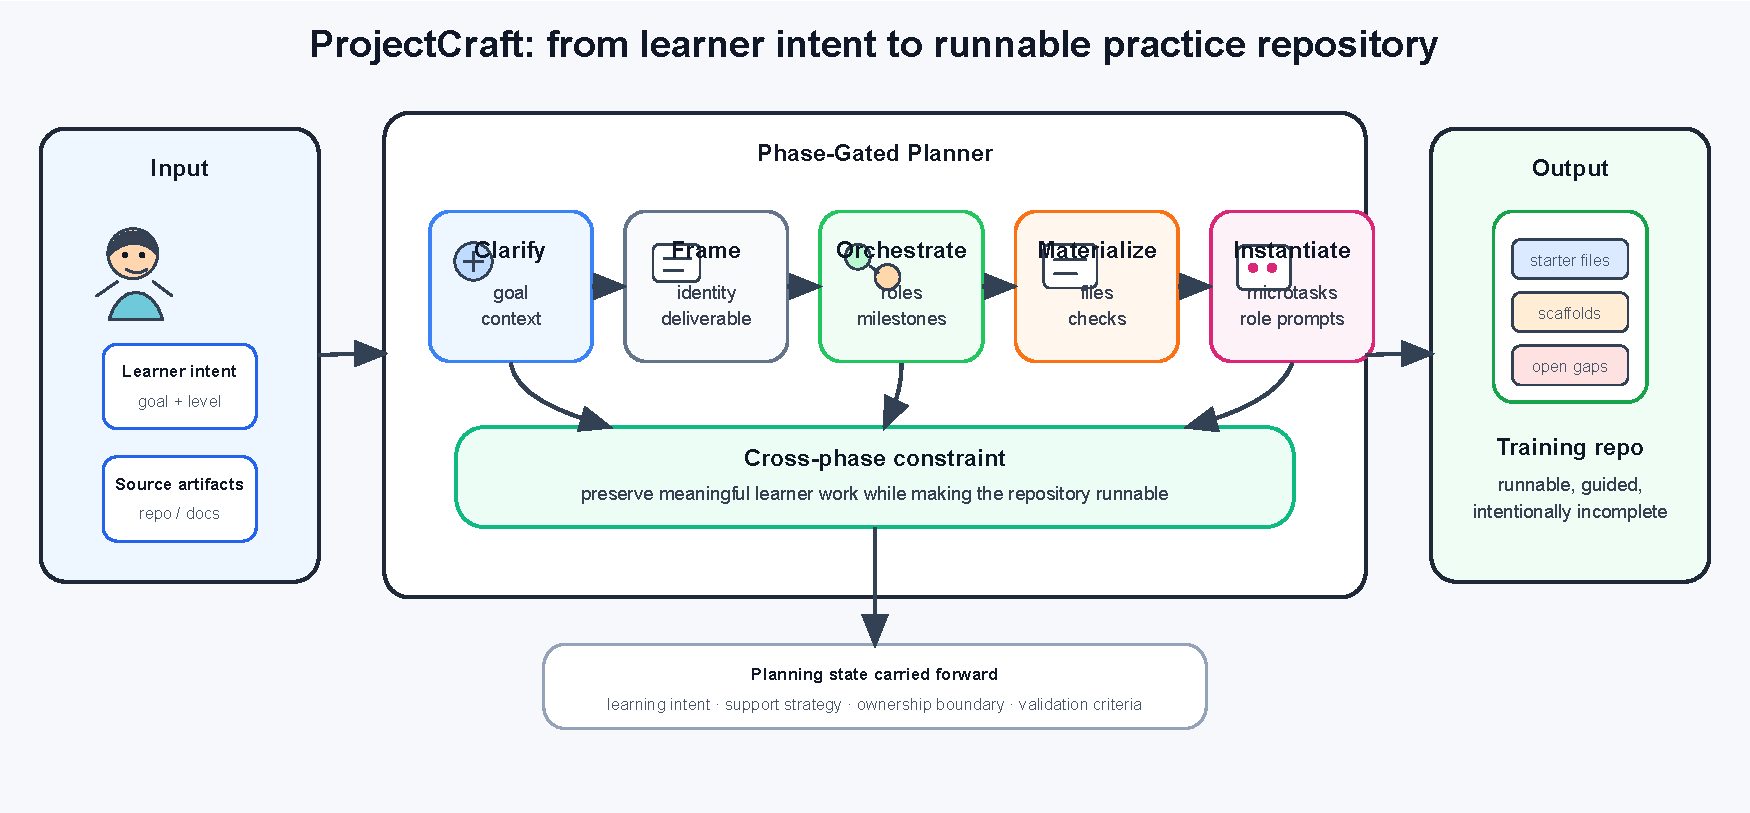
\includegraphics[width=\linewidth]{figures/method-overview.pdf}
    \caption{The phase-gated workflow of \model. The system progressively stabilizes learner intent, assignment identity, collaboration structure, concrete materials, and execution-ready microtasks while maintaining a cross-phase constraint that meaningful learner work remains learner-owned.}
    \label{fig:method-overview}
\end{figure}

In the \textit{Clarify} phase, \model interprets the learner's goal and available context.
Learning goals may be stated at different levels of specificity, ranging from a broad topic or source repository to a concrete project deliverable.
\model identifies the intended learning outcome, the available source context, and the learner's proficiency so that subsequent decisions can be calibrated to the learner rather than to a generic project template.
The output is a stabilized learning intent that anchors the remaining workflow.

In the \textit{Frame} phase, \model turns the stabilized intent into an assignment identity.
This includes the project goal, final deliverable, title, description, and topical tags.
The purpose of this phase is to make the assignment legible before detailed tasks or files are produced: the system first decides what the learner is working toward, then decides how that work should be organized.

In the \textit{Orchestrate} phase, \model designs the collaboration pattern for the assignment.
It creates milestones, introduces the roles needed to support the learner, and determines how responsibility should be distributed across learner work, instructor oversight, AI assistance, and optional scene interaction.
Every assignment includes a learner role and an instructor role.
Depending on the assignment type, \model may also introduce AI collaborators for implementation support, checking, research, or scaffolding, and scene actors for role-play settings such as interviews, negotiation, or communication practice.

In the \textit{Materialize} phase, \model generates the concrete resources needed for the assignment.
These include starter files, configuration files, fixtures, examples, learner documents, scaffolds, and validation resources.
This phase turns the assignment from a plan into a workspace context in which the learner can act.

In the \textit{Instantiate} phase, \model turns each milestone into execution-ready microtasks.
Each microtask specifies its goal, responsible role, participants, expected output, and role-specific guidance for execution.
The resulting assignment can then be reviewed by the learner and passed to the workspace execution phase, where the learner, instructor, AI collaborators, and optional scene actors interact around the generated tasks.

\subsection{Learning-Preserving Task Synthesis}

A key challenge in task synthesis is to make the generated project executable while preserving the learner work that carries the intended practice.
\model therefore distinguishes between core learning work and auxiliary work.
Core learning work includes decisions, implementations, analyses, or communications that directly exercise the target skill.
Auxiliary work includes setup, boilerplate, repetitive configuration, mechanical glue code, or contextual preparation that is necessary for execution but not central to the learning objective.
\model preserves core learning work for the learner, while assigning auxiliary work to system-generated materials or AI collaborators when doing so helps the learner focus on the intended skill.

Learner proficiency controls how this ownership boundary is drawn and how it appears in the generated assignment.
For beginners, \model uses smaller milestones, denser scaffolding, more explicit instructions, and greater system support for setup and navigation.
For intermediate learners, the system shares responsibility between learner work and AI assistance, preserving meaningful design and implementation choices while providing targeted support.
For advanced learners, \model leaves more architectural decisions, implementation gaps, and validation reasoning to the learner, while using AI roles mainly for feedback, review, and verification.
These choices are reflected in milestone granularity, task descriptions, starter-file gaps, scaffolds, and validation criteria, so learner adaptation changes the structure of the assignment rather than only the wording of the instructions.

\subsection{Repository Realization}

Repository realization turns the planned assignment into a concrete training repository.
Using the learning intent, support strategy, ownership boundary, and validation criteria determined in earlier phases, \model generates the materials needed for practice: starter files, requirements, examples, documents, scaffolds, and checks.
These materials give learners a concrete context in which to work, while the associated guidance records how that work should be supported and evaluated.

The resulting repository is designed to be runnable but not complete.
Starter materials provide the initial code, documents, and task context needed to begin the assignment.
When a source artifact such as a GitHub repository is available, \model uses it to derive realistic starter files, constraints, examples, and validation checks.
At the same time, \model leaves intentional gaps where learners should make decisions, implement functionality, conduct analysis, or produce communicative artifacts.
These gaps are chosen to exercise the target skill, so the repository remains a learning environment rather than a completed solution.
\model then generates tests, rubrics, or milestone checks based on the work the learner is expected to complete.
